\documentclass[aspectratio=169,11pt]{beamer}
\usetheme{default}
\usecolortheme{dove}
\usepackage{amsmath,amssymb,graphicx,tikz,pgfplots,booktabs}
\usetikzlibrary{arrows.meta,positioning,calc}
\pgfplotsset{compat=1.18}
\definecolor{DeckNavy}{HTML}{17324D}
\definecolor{DeckBlue}{HTML}{2D70B3}
\definecolor{DeckGreen}{HTML}{6F9940}
\definecolor{DeckRed}{HTML}{D95F4A}
\definecolor{DeckGold}{HTML}{D4A72C}
\definecolor{DeckGray}{HTML}{65727E}
\definecolor{DeckLight}{HTML}{F2F5F7}
\setbeamercolor{normal text}{fg=DeckNavy,bg=white}
\setbeamercolor{frametitle}{fg=DeckNavy,bg=white}
\setbeamercolor{title}{fg=DeckNavy}
\setbeamercolor{structure}{fg=DeckBlue}
\setbeamerfont{title}{size=\LARGE,series=\bfseries}
\setbeamerfont{frametitle}{size=\Large,series=\bfseries}
\setbeamertemplate{navigation symbols}{}
\setbeamertemplate{frametitle}{\vspace{0.25em}\hspace{0.15em}\insertframetitle\par
  \vspace{-0.35em}\hspace{0.15em}{\color{DeckGreen}\rule{1.3cm}{1.5pt}}}
\setbeamertemplate{footline}{\hfill\color{DeckGray}\scriptsize\insertframenumber\hspace{0.5cm}\vspace{0.2cm}}
\setbeamersize{text margin left=0.65cm,text margin right=0.65cm}
\hyphenpenalty=10000
\exhyphenpenalty=10000
\hypersetup{pdftitle={SGM Graph Filter Progress Update},pdfauthor={Harshil Shah},pdfsubject={Paper Reproduction, Torch Functions, and MLP Experiment}}
\newenvironment{canvas}{\begin{tikzpicture}[remember picture,overlay,shift={(current page.north west)},x=1cm,y=-1cm]}{\end{tikzpicture}}
\tikzset{txt/.style={anchor=north west,align=left,inner sep=0,text=DeckNavy},
  smalltxt/.style={txt,font=\small},
  labeltxt/.style={txt,font=\scriptsize,text=DeckGray},
  arr/.style={-{Latex[length=2mm]},thick,DeckGreen}}
\newcommand{\code}[1]{\texttt{\detokenize{#1}}}
\newcommand{\callout}[1]{\node[txt,fill=DeckNavy,text=white,rounded corners=2pt,
  inner sep=0.19cm,text width=13.8cm,align=center,font=\small\bfseries] at (0.9,7.20) {#1};}
\newcommand{\source}[1]{\node[labeltxt,text width=14.5cm,font=\tiny] at (0.75,8.12) {#1};}
\pgfplotsset{deckaxis/.style={axis lines=left,axis line style={DeckGray},
  tick label style={font=\scriptsize,text=DeckGray},label style={font=\small,text=DeckNavy},
  title style={font=\small\bfseries,text=DeckNavy},
  grid=major,grid style={DeckGray!14},tick style={DeckGray},
  legend style={draw=none,font=\scriptsize,fill=none},clip=true}}


\newcommand{\TanhPlot}{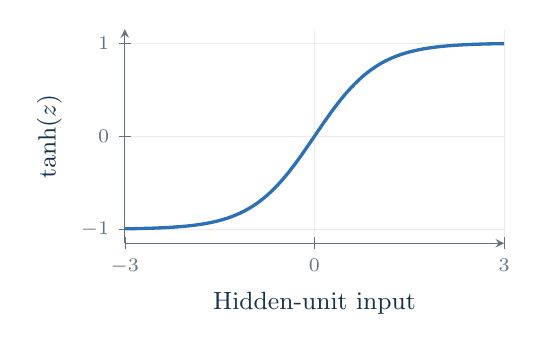
\begin{tikzpicture}\begin{axis}[deckaxis,width=6.4cm,height=4.3cm,xmin=-3,xmax=3,ymin=-1.15,ymax=1.15,xtick={-3,0,3},ytick={-1,0,1},xlabel={Hidden-unit input},ylabel={$\tanh(z)$}]\addplot[DeckBlue,very thick,domain=-3:3,samples=100] {tanh(x)};\end{axis}\end{tikzpicture}}

\begin{document}

\begin{frame}[plain,noframenumbering]
\begin{canvas}
  \node[txt,font=\LARGE\bfseries,text width=13.7cm] at (0.9,2.05)
    {SGM Graph Filter\\Progress Update};
  \draw[DeckGreen,line width=1.5pt] (0.9,3.7) -- (2.4,3.7);
  \node[txt,font=\large,text width=14cm] at (0.9,4.18)
    {Paper Reproduction, Torch Functions, and MLP Experiment};
  \node[smalltxt] at (0.9,5.45)
    {Harshil Shah\\[0.18cm]Mission San Jose High School\\[0.18cm]October 5, 2026};
\end{canvas}
\note{SGM means Spectral Graph Model. The reproduction uses supplied fitted parameters. A verified cohort MLP experiment has not been run.}
\end{frame}

% Four stages of the actual NumPy function, with equations on the left.
\begin{frame}[t]{\texttt{network\_transfer\_local\_alpha}}
\begin{canvas}
  \only<1>{
    \node[txt,font=\large\bfseries] at (0.85,1.55) {Propagation delay};
    \node[smalltxt,text width=6.2cm] at (0.85,2.55)
      {$\tau_{ij}=10^{-3}D_{ij}/v$\\[0.5cm]
       $C_{ij}(\omega)=C_{ij}e^{-i\omega\tau_{ij}}$\\[0.6cm]
       $C$: connection strengths\\[0.18cm]
       $D$: distances in mm\\[0.18cm]
       $v$: speed in m/s};
    \node[txt,font=\footnotesize] at (7.6,2.55) {\begin{tabular}{@{}l@{}}
      \code{C = brain.reducedConnectome}\\[0.24cm]
      \code{D = brain.distance_matrix}\\[0.45cm]
      \code{Tau = 0.001 * D / speed}\\[0.24cm]
      \code{Cc = C * np.exp(-1j * Tau * w)}
    \end{tabular}};
    \node[smalltxt,text width=14cm] at (0.85,7.0)
      {\code{run_local_coupling_forward} calls this function at each $\omega=2\pi f$.};
  }
  \only<2>{
    \node[txt,font=\large\bfseries] at (0.85,1.55) {Graph modes};
    \node[smalltxt,text width=6.2cm] at (0.85,2.5)
      {$L=I-\alpha\operatorname{diag}(d)C(\omega)$\\[0.5cm]
       $Lu_k=\lambda_k u_k$\\[0.5cm]
       $d$: inverse degree scaling\\[0.18cm]
       $\alpha$: coupling\\[0.18cm]
       $(\lambda_k,u_k)$: eigenvalue and eigenvector};
    \node[txt,font=\footnotesize] at (7.6,2.5) {\begin{tabular}{@{}l@{}}
      \code{L1 = np.identity(nroi)}\\[0.18cm]
      \code{L = L1 - alpha * np.matmul(}\\[0.10cm]
      \hspace{0.3cm}\code{np.diag(L2), Cc)}\\[0.3cm]
      \code{d, v = np.linalg.eig(L)}\\[0.18cm]
      \code{eig_ind = np.argsort(np.abs(d))}\\[0.18cm]
      \code{eig_vec = v[:, eig_ind]}\\[0.18cm]
      \code{eig_val = d[eig_ind]}\\[0.18cm]
      \code{eigenvectors = eig_vec[:, 0:K]}
    \end{tabular}};
  }
  \only<3>{
    \node[txt,font=\large\bfseries] at (0.85,1.55) {Local dynamics};
    \node[smalltxt,text width=6.4cm] at (0.85,2.4)
      {$F_e=\dfrac{1}{(1+i\omega\tau_e)^2},\quad
        F_i=\dfrac{g_{ii}}{(1+i\omega\tau_i)^2}$\\[0.32cm]
       $H_{ed}=\dfrac{\alpha/\tau_e}{i\omega+(\alpha/\tau_e)F_e}$\\[0.22cm]
       $H_{id}=\dfrac{\alpha/\tau_i}{i\omega+(\alpha/\tau_i)F_i}$\\[0.22cm]
       $H_{eid}=\dfrac{g_{ei}F_eF_i}{1+g_{ei}F_eF_i}$\\[0.22cm]
       $H_{\mathrm{total}}=aH_{ed}+\dfrac{1-a}{2}(H_{id}+H_{eid})$};
    \node[txt,font=\footnotesize] at (7.6,2.4) {\begin{tabular}{@{}l@{}}
      \code{Fe = np.divide(1 / tau_e ** 2,}\\[0.08cm]
      \hspace{0.3cm}\code{(1j * w + 1 / tau_e) ** 2)}\\[0.20cm]
      \code{Fi = np.divide(gii * 1 / tau_i ** 2,}\\[0.08cm]
      \hspace{0.3cm}\code{(1j * w + 1 / tau_i) ** 2)}\\[0.20cm]
      \code{Hed = alpha / tau_e / (}\\[0.08cm]
      \hspace{0.3cm}\code{1j * w + alpha / tau_e * Fe)}\\[0.20cm]
      \code{Hid = alpha / tau_i / (}\\[0.08cm]
      \hspace{0.3cm}\code{1j * w + alpha / tau_i * Fi)}\\[0.20cm]
      \code{Heid = gei * Fe * Fi / (1 + gei * Fe * Fi)}\\[0.2cm]
      \code{Htotal = (a * Hed + (1 - a) / 2 * Hid}\\[0.08cm]
      \hspace{0.3cm}\code{+ (1 - a) / 2 * Heid)}
    \end{tabular}};
  }
  \only<4>{
    \node[txt,font=\large\bfseries] at (0.85,1.55) {Regional response};
    \node[smalltxt,text width=6.3cm] at (0.85,2.4)
      {$q_k=\dfrac{i\omega\tau_C}{\alpha}+F_e\lambda_k$\\[0.42cm]
       $\widetilde q_k=\max(|q_k|,\,0.05\max_j|q_j|)e^{i\arg(q_k)}$\\[0.42cm]
       $R_k=H_{\mathrm{total}}/\widetilde q_k$\\[0.42cm]
       $\widehat x_r=\displaystyle\sum_{k=1}^{K-1}u_{rk}R_k$\\[0.32cm]
       Mode 0 is omitted.};
    \node[txt,font=\footnotesize] at (7.6,2.4) {\begin{tabular}{@{}l@{}}
      \code{q1 = 1 / alpha * tauC * (}\\[0.08cm]
      \hspace{0.3cm}\code{1j * w + alpha / tauC * Fe * eigenvalues)}\\[0.2cm]
      \code{qthr = zero_thr * np.abs(q1[:]).max()}\\[0.13cm]
      \code{magq1 = np.maximum(np.abs(q1), qthr)}\\[0.13cm]
      \code{angq1 = np.angle(q1)}\\[0.13cm]
      \code{q1 = np.multiply(magq1, np.exp(1j * angq1))}\\[0.13cm]
      \code{frequency_response = np.divide(Htotal, q1)}\\[0.25cm]
      \code{model_out = 0}\\[0.13cm]
      \code{for k in range(1, K):}\\[0.08cm]
      \hspace{0.3cm}\code{model_out += frequency_response[k] * (}\\[0.08cm]
      \hspace{0.6cm}\code{eigenvectors[:, k])}
    \end{tabular}};
  }
\end{canvas}
\note{Equations describe the repository local-alpha function. They are algebraically equivalent to the displayed source excerpts. Degree scaling uses inverse square root of rowdegree times coldegree plus machine epsilon, with low-degree nodes masked to zero scaling. The code sorts by absolute eigenvalue and skips zero-indexed mode 0. The wrapper run_local_coupling_forward sweeps angular frequency 2*pi*f.}
\end{frame}

\begin{frame}[t]{Paper Reproduction}
\begin{canvas}
  \only<1>{
    \node[txt,font=\large\bfseries] at (0.85,1.5) {What I ran for this update};
    \node[smalltxt,text width=14cm] at (0.85,2.15)
      {The forward calculation from \code{spectral_correlation.ipynb}.};
    \node[smalltxt,text width=6.3cm] at (0.85,3.6)
      {\textbf{Inputs}\\[0.3cm]Saved parameter fits\\[0.18cm]Connectomes and MEG spectra\\[0.18cm]68 MEG regions, 40 frequencies};
    \draw[arr] (7.05,4.55) -- (8.0,4.55);
    \node[smalltxt,text width=6.4cm] at (8.4,3.6)
      {\textbf{Outputs}\\[0.3cm]Predicted regional spectra\\[0.18cm]Spectral correlations\\[0.32cm]
       \textcolor{DeckGreen}{\textbf{36/36 matched}} the saved scores};
  }
  \only<2>{
    \node[txt] at (1.35,1.4)
      {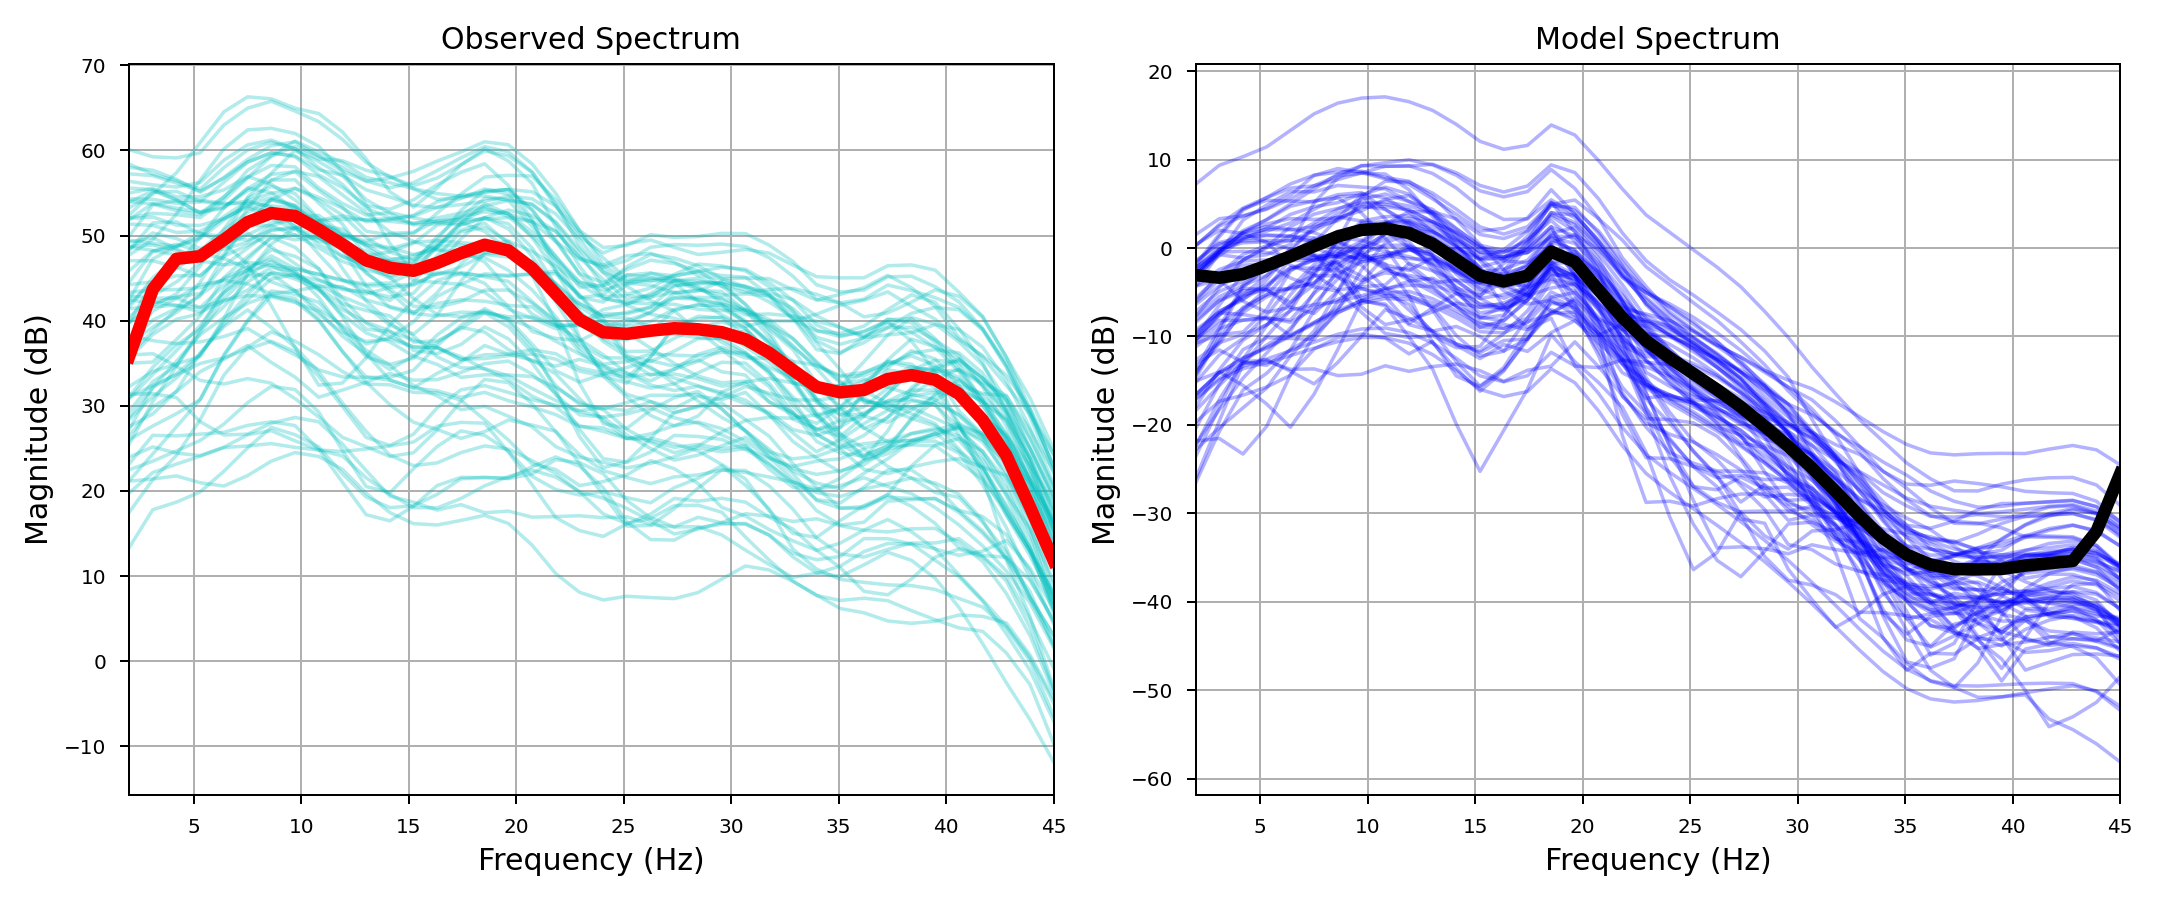
\includegraphics[width=13.2cm]{../figures/replay-spectrum.png}};
    \node[smalltxt,text width=14cm] at (0.85,7.0)
      {Figure 3 comparison: observed and modeled spectra from the replay.};
    \node[labeltxt,text width=14cm] at (0.85,7.55)
      {Retained record 1, using the notebook plotting method.};
  }
\end{canvas}
\note{Paper https://pmc.ncbi.nlm.nih.gov/articles/PMC7336150/ Figures 3 and 4c are corresponding analyses. The 36/36 check compares replayed cohort scores with individualC_optP.mat within 1e-9. The figure shows retained record 1 from the current historical cohort replay, selected previously as the lower median correlation. A single-record forward rerun verified the displayed data against figures/historical_spectra.npz. It uses individual connectivity at historical compacted index 0 and the corresponding retained MEG and fitted parameters. The plotting operations follow reproduce_MEG_spectra.ipynb: magnitude smoothing and dB conversion, all 68 regions, and red/black mean curves. No extra normalization. Full source hashes and checks are in figures/replay-spectrum-provenance.json.}
\end{frame}

\begin{frame}[t]{What still needs to be confirmed?}
\begin{canvas}
  \only<1>{
    \node[txt,font=\large\bfseries,text width=14cm] at (0.85,1.65) {Do we need a subject map to match these files?};
    \node[smalltxt,text width=4.1cm] at (0.85,2.65)
      {\textbf{Connectomes}\\[0.3cm]39 records\\[0.16cm]No subject IDs};
    \node[smalltxt,text width=4.1cm] at (5.9,2.65)
      {\textbf{Fitted parameters}\\[0.3cm]36 nonempty records};
    \node[smalltxt,text width=4.1cm] at (10.9,2.65)
      {\textbf{MEG spectra}\\[0.3cm]36 nonempty records};
    \draw[DeckGray,dashed,thick] (4.5,3.3) -- (5.45,3.3);
    \draw[DeckGray,dashed,thick] (9.9,3.3) -- (10.45,3.3);
    \node[smalltxt,text width=14cm] at (0.85,5.2)
      {Need to confirm which connectome goes with each MEG record and parameter set.};
  }
  \only<2>{
    \node[smalltxt,text width=6.3cm] at (0.85,2.0)
      {\textbf{Region matching}\\[0.4cm]
       82 structural nodes\\[0.08cm]
       {\scriptsize (\code{individual_subjects.mat})}\\[0.3cm]
       86 model nodes\\[0.08cm]
       {\scriptsize (\code{OrderingAlphabetical_86ROIs.txt})}\\[0.3cm]
       68 MEG regions\\[0.08cm]
       {\scriptsize (\code{freqMEGdata.mat})}\\[0.5cm]
       \textbf{Need the ordered region map.}};
    \node[smalltxt,text width=6.3cm] at (8.4,2.0)
      {\textbf{Remaining reproduction}\\[0.4cm]
       Fresh parameter fitting\\[0.25cm]
       Spatial alpha/beta results};
  }
\end{canvas}
\note{Empty parameter and MEG indices are 21,22,28, zero-based. The indexing discrepancy does not identify the true order of the unlabeled structural records. Subject mapping, ordered atlas labels and frequency metadata require confirmation before generating a training cache. Reproducing saved scores does not resolve these identities.}
\end{frame}

\begin{frame}[t]{Torch Functions}
\begin{canvas}
  \only<1>{
    \node[smalltxt,text width=6.8cm] at (0.85,2.0)
      {\textbf{NumPy source}\\[0.4cm]
       \code{network_transfer_local_alpha}\\[0.35cm]
       \code{run_local_coupling_forward}};
    \node[smalltxt,text width=6.7cm] at (8.0,2.0)
      {\textbf{Torch counterparts}\\[0.4cm]
       {\footnotesize\code{network_transfer_local_alpha_torch}}\\[0.35cm]
       {\footnotesize\code{run_local_coupling_forward_torch}}};
    \node[smalltxt,text width=14cm] at (0.85,5.1)
      {Inside the Torch forward function:\\[0.35cm]
       \code{prepare_graph_torch}\quad computes the graph modes.\\[0.3cm]
       \code{evaluate_response_torch}\quad computes the response.};
  }
  \only<2>{
    \node[txt,font=\large\bfseries] at (0.85,1.55) {\code{prepare_graph_torch}};
    \node[smalltxt,text width=6.1cm] at (0.85,2.5)
      {$C_{ij}(\omega)=C_{ij}e^{-i\omega\tau_{ij}}$\\[0.45cm]
       $L=I-\alpha\operatorname{diag}(d)C(\omega)$\\[0.45cm]
       $Lu_k=\lambda_k u_k$};
    \node[txt,font=\footnotesize] at (7.6,2.5) {\begin{tabular}{@{}l@{}}
      \code{Tau = 0.001 * D / speed}\\[0.2cm]
      \code{Cc = C * torch.exp(-1j * Tau * w)}\\[0.28cm]
      \code{values, vectors = torch.linalg.eig(L)}\\[0.2cm]
      \code{order = torch.argsort(torch.abs(values))}\\[0.2cm]
      \code{eigenvalues = values[order]}\\[0.2cm]
      \code{eigenvectors = vectors[:, order][:, :K]}
    \end{tabular}};
    \node[labeltxt,text width=14cm] at (0.85,6.9)
      {Same degree scaling and mode order. Each eigenvector's largest entry is made positive real to fix its phase.};
  }
  \only<3>{
    \node[txt,font=\large\bfseries] at (0.85,1.55) {\code{evaluate_response_torch}};
    \node[smalltxt,text width=6.1cm] at (0.85,2.55)
      {$F_e^{\mathrm{local}}=\dfrac{1}{(1+i\omega\tau_e)^2}$\\[0.48cm]
       $H_{ed}=\dfrac{\alpha/\tau_e}{i\omega+(\alpha/\tau_e)F_e^{\mathrm{local}}}$\\[0.48cm]
       $H_{eid}=\dfrac{g_{ei}F_e^{\mathrm{local}}F_i}{1+g_{ei}F_e^{\mathrm{local}}F_i}$};
    \node[txt,font=\footnotesize] at (7.6,2.55) {\begin{tabular}{@{}l@{}}
      \code{Fe_local = (1 / tau_e**2) / (}\\[0.1cm]
      \hspace{0.3cm}\code{1j * w + 1 / tau_e) ** 2}\\[0.35cm]
      \code{Hed = (alpha / tau_e) / (}\\[0.1cm]
      \hspace{0.3cm}\code{1j * w + alpha / tau_e * Fe_local)}\\[0.35cm]
      \code{Heid = gei * Fe_local * Fi / (}\\[0.1cm]
      \hspace{0.3cm}\code{1 + gei * Fe_local * Fi)}
    \end{tabular}};
    \node[labeltxt,text width=14cm] at (0.85,6.9)
      {The local excitatory and inhibitory equations keep the NumPy algebra.};
  }
  \only<4>{
    \node[txt,font=\large\bfseries,text=DeckBlue] at (0.85,1.85) {Local dynamics};
    \node[smalltxt,text width=6.3cm] at (0.85,2.7)
      {$F_e^{\mathrm{local}}(\omega)=\dfrac{1}{(1+i\omega\tau_e)^2}$\\[0.45cm]
       Enters $H_{ed}$ and $H_{eid}$.\\[0.3cm]
       Uses the subject's fitted $\tau_e$.};
    \node[txt,font=\large\bfseries,text=DeckGreen] at (8.0,1.85) {Graph propagation};
    \node[smalltxt,text width=6.8cm] at (8.0,2.7)
      {$q_k=\dfrac{i\omega\tau_C}{\alpha}+F_e^{\mathrm{graph}}\lambda_k$};
    \node[txt,font=\footnotesize] at (8.0,3.9) {\begin{tabular}{@{}l@{}}
      \code{if Fe_graph is None:}\\[0.14cm]
      \hspace{0.3cm}\code{Fe_graph = Fe_local}\\[0.32cm]
      \code{q1 = (tauC / alpha) * (}\\[0.10cm]
      \hspace{0.3cm}\code{1j * w + alpha / tauC * Fe_graph}\\[0.10cm]
      \hspace{0.3cm}\code{* graph["eigenvalues"])}
    \end{tabular}};
    \node[smalltxt,text width=14cm] at (0.85,7.2)
      {The MLP will replace \code{Fe_graph}. Local dynamics stay analytical.};
  }
\end{canvas}
\note{The wrapper prepares graph eigenpairs and evaluates the response. Cache reuse requires fixed connectivity, distances, angular frequency, alpha, speed and mode selection. Eigenvector phase is fixed before the phase-sensitive modal sum. The analytical graph filter defaults to Fe_local. Supplying Fe_graph changes only the graph denominator. Checks from the prior build: 14 passed and one failed because a rejection test expected unverified while the raised text was not verified. See figures/test-results.txt. Numerical parity details remain in figures/evidence.json. No model source was changed for this revision.}
\end{frame}

\begin{frame}[t]{MLP Implemented So Far}
\begin{canvas}
  \only<1>{
    \node[smalltxt,text width=6.8cm] at (0.85,1.9)
      {\textbf{\code{training/filters.py}}\\[0.4cm]
       \code{generate_training_data}\\[0.16cm]
       Saves graph modes, parameters and MEG.\\[0.4cm]
       \code{FeGraphMLP}\\[0.16cm]
       Maps frequency to one complex filter value.\\[0.4cm]
       \code{predict_spectra}\\[0.16cm]
       Uses the saved graphs and filter values.};
    \node[smalltxt,text width=6.3cm] at (8.4,1.9)
      {\textbf{\code{training/train.py}}\\[0.4cm]
       \code{train_filter}\\[0.16cm]
       Trains the shared MLP.\\[0.4cm]
       Validation selects the saved weights.\\[0.4cm]
       Saves loss history and split scores.};
  }
  \only<2>{
    \node[txt,font=\large\bfseries] at (0.85,1.55) {\code{FeGraphMLP}};
    \node[smalltxt,text width=3.4cm,align=center] at (0.8,2.8)
      {\textbf{Input}\\[0.4cm]
       Frequency $\omega$\\[0.28cm]
       Scaled by $2\pi\cdot45$};
    \draw[arr] (4.25,3.65) -- (4.95,3.65);
    \node[smalltxt,text width=4.7cm,align=center] at (5.05,2.8)
      {\textbf{Hidden layers}\\[0.4cm]
       Configurable number and width\\[0.28cm]
       Current setting: 1 layer, 8 units\\[0.28cm]
       Activation: $\tanh$};
    \draw[arr] (9.85,3.65) -- (10.55,3.65);
    \node[smalltxt,text width=4.2cm,align=center] at (10.6,2.8)
      {\textbf{Output}\\[0.4cm]
       Two real values\\[0.28cm]
       $\operatorname{Re}F_\theta,\ \operatorname{Im}F_\theta$};
    \node[smalltxt,text width=14cm,align=center] at (0.85,6.3)
      {$F_\theta(\omega)=\operatorname{Re}F_\theta(\omega)+i\operatorname{Im}F_\theta(\omega)$\\[0.35cm]
       One learned complex graph-filter value per frequency, shared across subjects.};
  }
\end{canvas}
\note{Source: spectrome/training/filters.py and train.py. FeGraphMLP accepts a tuple of hidden layer widths through hidden_sizes. Each hidden layer uses Tanh and the last layer is linear with two outputs. The complex filter is assembled from these real and imaginary components. generate_training_data saves graph modes and data with provenance; train_filter saves weights selected by validation and split scores. Data mapping remains unresolved and no cohort learning result is claimed.}
\end{frame}

\begin{frame}[t]{Preliminary Implementation Choices}
\begin{canvas}
  \node[txt,font=\large\bfseries] at (0.85,1.65) {$\tanh$ activation};
  \node[txt] at (0.7,2.5) {\TanhPlot};
  \node[labeltxt,text width=6.2cm] at (0.85,7.15)
    {Smooth hidden activation. The final linear layer leaves the output unbounded.};
  \node[smalltxt,text width=6.3cm] at (8.4,1.85)
    {\textbf{Starter architecture}\\[0.4cm]
     1 input: scaled frequency\\[0.28cm]
     1 hidden layer: 8 units\\[0.28cm]
     2 outputs: real and imaginary parts\\[0.28cm]
     34 trainable parameters\\[0.5cm]
     Frequency scale: $2\pi\cdot45$ rad/s};
  \node[labeltxt,text width=6.3cm] at (8.4,6.8)
    {Adam, learning rate $10^{-3}$\\[0.12cm]100 epochs, seed 7};
\end{canvas}
\note{Architecture is 1 to 8 to 2, with 8+8+16+2=34 trainable parameters. Tanh is smooth and bounded internally, while the final linear output is unbounded. Smoothness is a design motivation, not evidence of better fit or a guarantee of causal or stable dynamics. Input scaling is 2*pi*45 rad/s.}
\end{frame}

\begin{frame}[t]{MLP Training}
\begin{canvas}
    \node[txt,font=\large\bfseries] at (0.85,1.55) {\code{train_filter}};
    \node[smalltxt,text width=6.1cm] at (0.85,2.55)
      {$\mathcal L=1-\dfrac{1}{S}\sum_{s=1}^{S}r_s$\\[0.5cm]
       $r_s$: mean regional spectral correlation\\[0.22cm]
       $S$: number of training subjects\\[0.5cm]
       Only the MLP weights are updated.\\[0.25cm]
       Graph modes are prepared once.};
    \node[txt,font=\footnotesize] at (7.6,2.55) {\begin{tabular}{@{}l@{}}
      \code{optimizer.zero_grad()}\\[0.25cm]
      \code{train_scores = correlations(}\\[0.13cm]
      \hspace{0.3cm}\code{splits["train"], model(omega))}\\[0.25cm]
      \code{loss = 1 - train_scores.mean()}\\[0.25cm]
      \code{loss.backward()}\\[0.25cm]
      \code{optimizer.step()}
    \end{tabular}};

\end{canvas}
\note{Source: spectrome/training/train.py. Each epoch is one full training-cohort Adam update, with only MLP weights trainable and graph modes cached. The loss uses magnitude, five-bin smoothing, square root with a 1e-12 floor and frequency demeaning. Validation selects the checkpoint before test scoring. The real cohort run still requires verified subject and region mappings.}
\end{frame}

\begin{frame}[t]{Planned Experiment}
\begin{canvas}
  \only<1>{
    \node[smalltxt,text width=6.4cm] at (0.85,2.0)
      {\textbf{Analytical graph filter}\\[0.4cm]
       $F_{e,s}(\omega)=\dfrac{1}{(1+i\omega\tau_{e,s})^2}$\\[0.4cm]
       Each subject's fitted time constant.};
    \node[smalltxt,text width=6.4cm] at (8.4,2.0)
      {\textbf{Learned graph filter}\\[0.4cm]
       $F_\theta(\omega)\in\mathbb C$\\[0.4cm]
       One MLP shared across subjects.};
    \node[smalltxt,text width=14cm] at (0.85,5.7)
      {Keep the subjects, SGM parameters, local dynamics and scoring fixed.\\[0.4cm]
       Compare spectral correlation on held-out subjects.};
  }
\end{canvas}
\note{This tests a learned shared graph filter conditional on fixed, previously MEG-fitted SGM parameters. It does not establish prediction from structural data alone on unseen subjects. Activation or width comparisons are proposed follow-ups with matched data splits, seeds and training budget. Spatial alpha/beta evaluation remains to be agreed.}
\end{frame}

\end{document}
